\documentclass{article}
\usepackage[a4paper, total={6in, 8in}]{geometry}
\usepackage{graphicx}
\usepackage{url}
\usepackage{natbib}
\usepackage{todonotes}
\usepackage{booktabs}
\usepackage{lineno}
\usepackage{color}
\usepackage{auto-pst-pdf}
\usepackage[colaction]{multicol}
\usepackage{caption}
\usepackage{svg}

\linespread{1.5}

\makeatletter
\renewcommand{\maketitle}{\bgroup\setlength{\parindent}{0pt}
	\begin{flushleft}
		
		{\huge\textbf{\@title}}
		
		\bigskip
		
 		{\large\textbf{\@author}}
	\end{flushleft}\egroup
}
\makeatother

\newcommand{\multicollinenumbers}{
	\linenumbers
	\def\makeLineNumber{\docolaction
		{\makeLineNumberLeft}
		{}
		{\makeLineNumberRight}
		}
}

\newenvironment{figurehere}
	{\def\@captype{figure}}
	{}

% Title
\title{A Topic Model of Climate Change Literature}
\title{Words, words, words: Mapping the Matter of Climate Change Literature}
\title{A Topography of Climate Change Research}
\author{Max Callaghan}


\begin{document}
\maketitle


\begin{linenumbers}

\noindent\textbf{	
The massive expansion of scientific literature on climate change challenges the Intergovenmental Panel on Climate Change (IPCC)'s ability to assess the science according to its objectives. 
Moreover, the number and variety of papers hinders researchers of the science-policy interface from making objective judgements about those IPCC assessments. In this paper, we present a novel application of a machine-reading approach to model the topical content of papers on climate change. This dynamic topic model provides the basis for a \textit{topography} of climate change literature. The thematic development of the field is outlined and used to inform an analysis of the topics which are better and less well covered by IPCC reports.
}



\bigskip

%\begin{multicols}{2}
	
%\multicollinenumbers
\bigskip
\noindent\textbf{To deal with the wicked problem of climate change, international policy-makers need the IPCC. The IPCC as map-makers.}

The IPCC sees its role as to ``assess on a comprehensive, objective, open and transparent basis the scientific, technical and socio-economic information relevant to [...] climate change'' \citep{IPCC2013}. Climate science is so broad, multi-disciplinary, and laden with uncertainties and values, that the role of the IPCC as assessment maker is vitally important to developing evidence-based international climate policy.
Making maps \citep{Edenhofer2015}



\bigskip
\noindent\textbf{The task of the IPCC has become much more difficult with big literature}

Further, it has been pointed out that, in the age of ``big literature'', providing assessments that are comprehensive, objective and transparent has become much more difficult \citep{Minx2017l}. 

When IPCC's citations constitute an ever-decreasing proportion of the totality of science on climate change, questions about the map that the IPCC reports produce become more pressing:

- Is the map up to date? Is it complete? Is the perspective representative? 



%%%%%

\bigskip
\noindent\textbf{The IPCC, its reports and processes have been the object of study before. These are also hampered by problems of scale though}

Various researchers have attempted to do empirical research on the assessment reports, and processes of inter. alia. the IPCC \citep{jabbour2017} \citep{Bjurström2011} \citep{Hulme2016}. 

Policy makers, when asked about their interactions with the IPCC call for a greater focus on solutions \citep{Kowarsch2017}

These studies are similarly challenged by the the size of the literature. Traditional bibliometric techniques are insufficient.

\bigskip
\noindent\textbf{Some literature exists on bibliometrics and climate change, but tends not to deal with text}

Bibliometrics e.g. \citep{Haunschild2016} \citep{Grieneisen2011}

Text based approaches are usually of a smaller scope \citep{Grubert2016} or methodological contributions \citep{Blei2003}


\bigskip
\noindent\textbf{The scale of the problem in context}

The scale of the challenge is depicted in figure \ref{growth}. Less than two thousand documents relevant to climate change were published before the first assessment report (see Methods for data, exclusions and processing). These documents contained 3,528 unique terms, each of which was used on average in 0.49\% of documents. In the three complete years since the publication of AR5, 128,357 documents have been published, containing 86,419 unique terms, used on average in 0.12\% of documents. To put this into context, the 1,189 chapters of the Bible contain a vocabulary of 11,977 unique words. Put another way, the 236,634 publications published in AR5 and AR6 are significantly larger than the 178,118 publications recorded in the first volume of the `Catalogue of Scientific Papers', compiled by the Royal Society to record the entirety of scientific output from 1800 to 1863 \citep{Csiszar2017}



\begin{figure}
	\begin{center}
		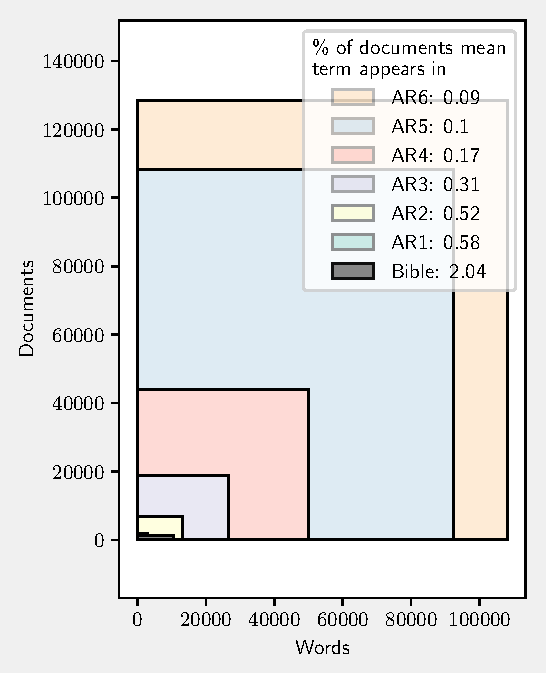
\includegraphics[width=0.5\linewidth]{plots/literature_size/volume_variety.pdf}
		%\captionof{figure}
		\caption{The volume and variety of literature on climate change has grown to unmanageable proportions. Each box represents a document-term matrix (unique documents x unique terms) of the abstracts written in each assessment period. The percentage of documents in which the average word occurs in is given in the key.
		}
		\label{growth}
	\end{center}
\end{figure}


\bigskip
\noindent\textbf{Machine reading to deal with scale problems in the making and assessing of maps}
	

Clearly, if the IPCC is to continue producing comprehensive assessments, it has to engage in machine-reading in order to remain anchored to the wider literature. Without such an approach, it becomes harder to justify which ever-diminishing proportion of the wider literature is included in assessments. Similarly, it becomes harder to criticise, with quantitatively evidenced claims, the outcomes of assessment processes.


\bigskip
\noindent\textbf{Dimension reduction makes possible the description in reduced form, and with less human bias, of unmanageably large datasets}

\citep{Greene2016} \citep{Lee1999}

This reduced form description makes comparisons more useful, when cutting the dataset.

\bigskip
\noindent\textbf{Machine reading is a supplement to assessment-making and not free from bias; a topography is not a map}

Machine reading approaches can of course not replace the task of human assessment-making. The contribution that could be made, though, is to pre-process the literature, producing a topographical map, used to navigate the literature while producing a more detailed assessment with human judgement.[[]] In fact this happens already - when IPCC authors search for literature on a topic, the results which appear on the search engine they use will be subject to algorithms based on the processing of millions of records of article text and metadata. This can be done in a much more systematic way when scientists perform directed analyses of the literature at scale.


\bigskip
\noindent\textbf{This study's contribution. Overarching themes, structure of the literature, development, relation to IPCC}

This study demonstrates how dynamic topic modelling can be used to gain an overview of an otherwise unmanageably large body of literature. This overview, or topography, describes the thematic development of the climate change literature and, in a novelly systematic way, examines how  comprehensively the IPCC has been able to engage with it. In pulling together strands from text-mining, bibliometrics, and the study of science and policy, this study advances our understanding of the literature on climate change and the role of the IPCC in communicating this to policy makers.


\section*{Results}

\bigskip
\noindent\textbf{A topographical map of climate change documents shows the broad structure of climate change literature}

Topics cut across both disciplinary, and working group lines - but disciplinary and working group structure remains visible in the map.

\begin{figure}
	\begin{center}
		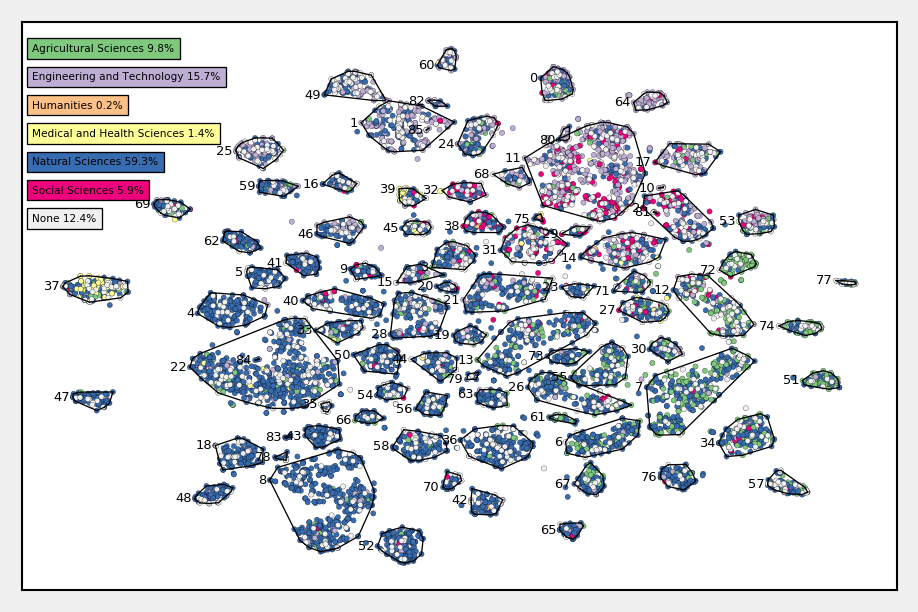
\includegraphics[width=1\linewidth]{plots/tsne.png}
		\caption{A map of a sample of 10,000 documents about climate change. Document positions are obtained by reducing the topic scores to two dimensions via t-SNE}
		\label{}
	\end{center}
\end{figure}

\begin{figure}
	\begin{center}
		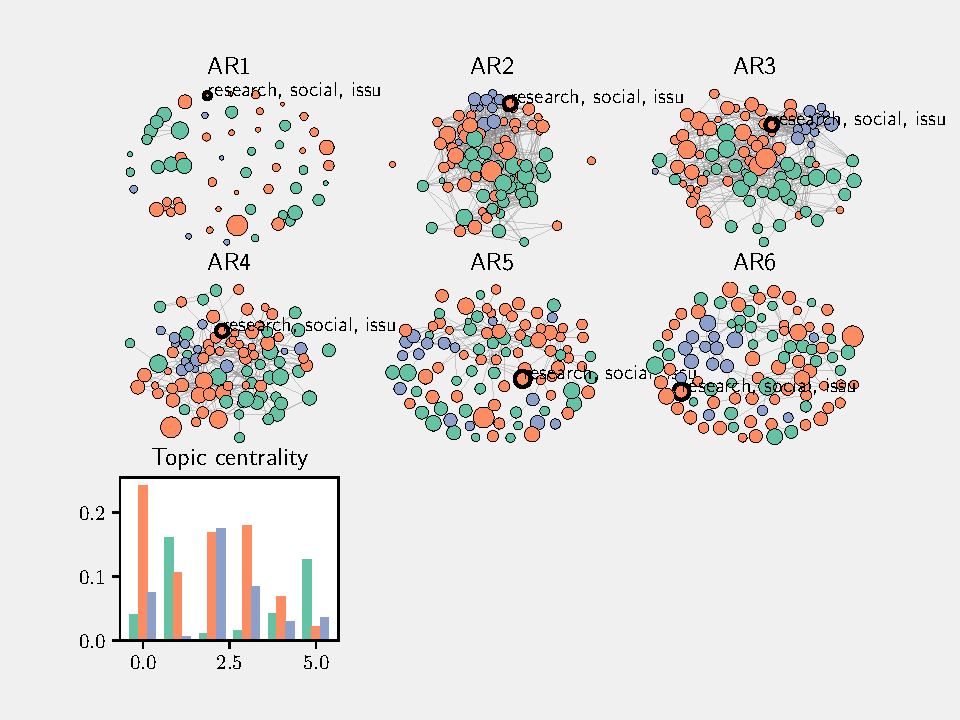
\includegraphics[width=1\linewidth]{plots/network_development_wgs_665.pdf}
		\caption{The development of the topic-document correlation network over IPCC assessment periods.}
		\label{}
	\end{center}
\end{figure}

\bigskip
\noindent\textbf{The topic-document correlation network is densest in AR2 and 3 but becomes more fragmented over time}

(partly: Model less good at describing literature later on)

\bigskip
\noindent\textbf{Working groups are clustered together [dynamics], with topics like [x] containing documents across working groups and topics like [y] important network nodes}


\begin{figure}
	\begin{center}
		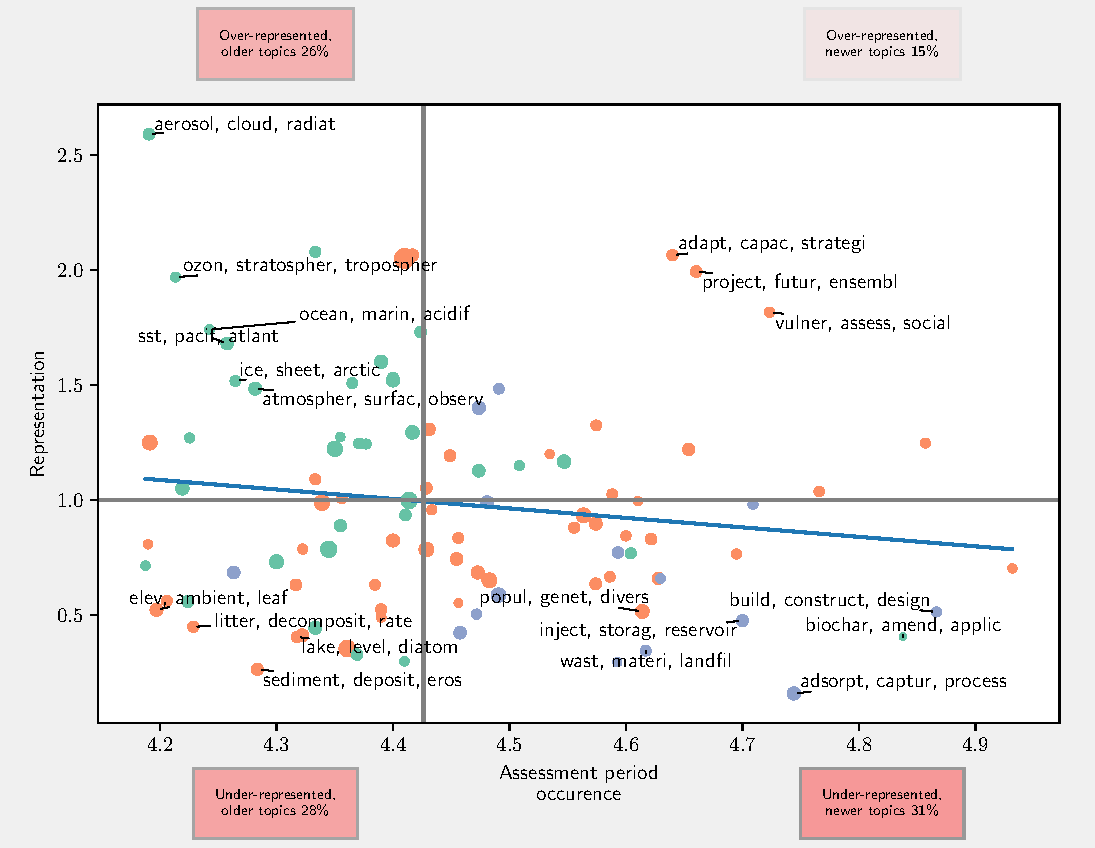
\includegraphics[width=1\linewidth]{plots/ipcc_representation/ipcc_rep_new665_all.pdf}
		\caption{Representation and newness of dynamic topics}
		\label{}
	\end{center}
\end{figure}


\bigskip
\noindent\textbf{Sustainability has been an increasingly important theme in an overarching topic about environmental sciences}

(compare to biochar, which is much more recent)

\begin{figure}
	\begin{center}
		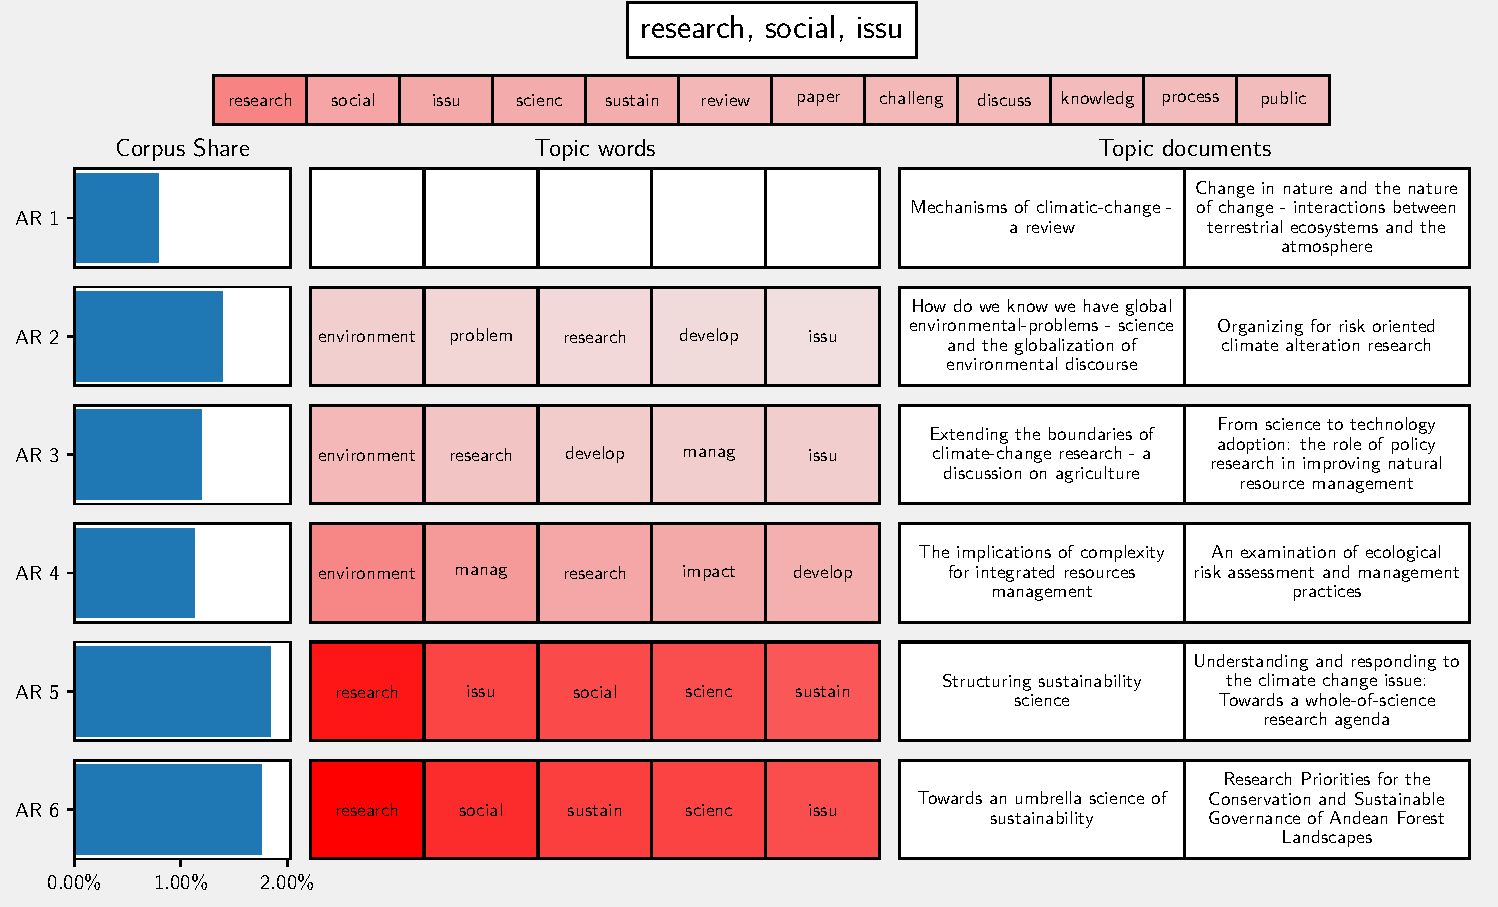
\includegraphics[width=1\linewidth]{plots/single_topic_3_11046.pdf}
		\caption{Word and document development of the ``Research'' dynamic topic}
		\label{}
	\end{center}
\end{figure}

\begin{figure}
	\begin{center}
		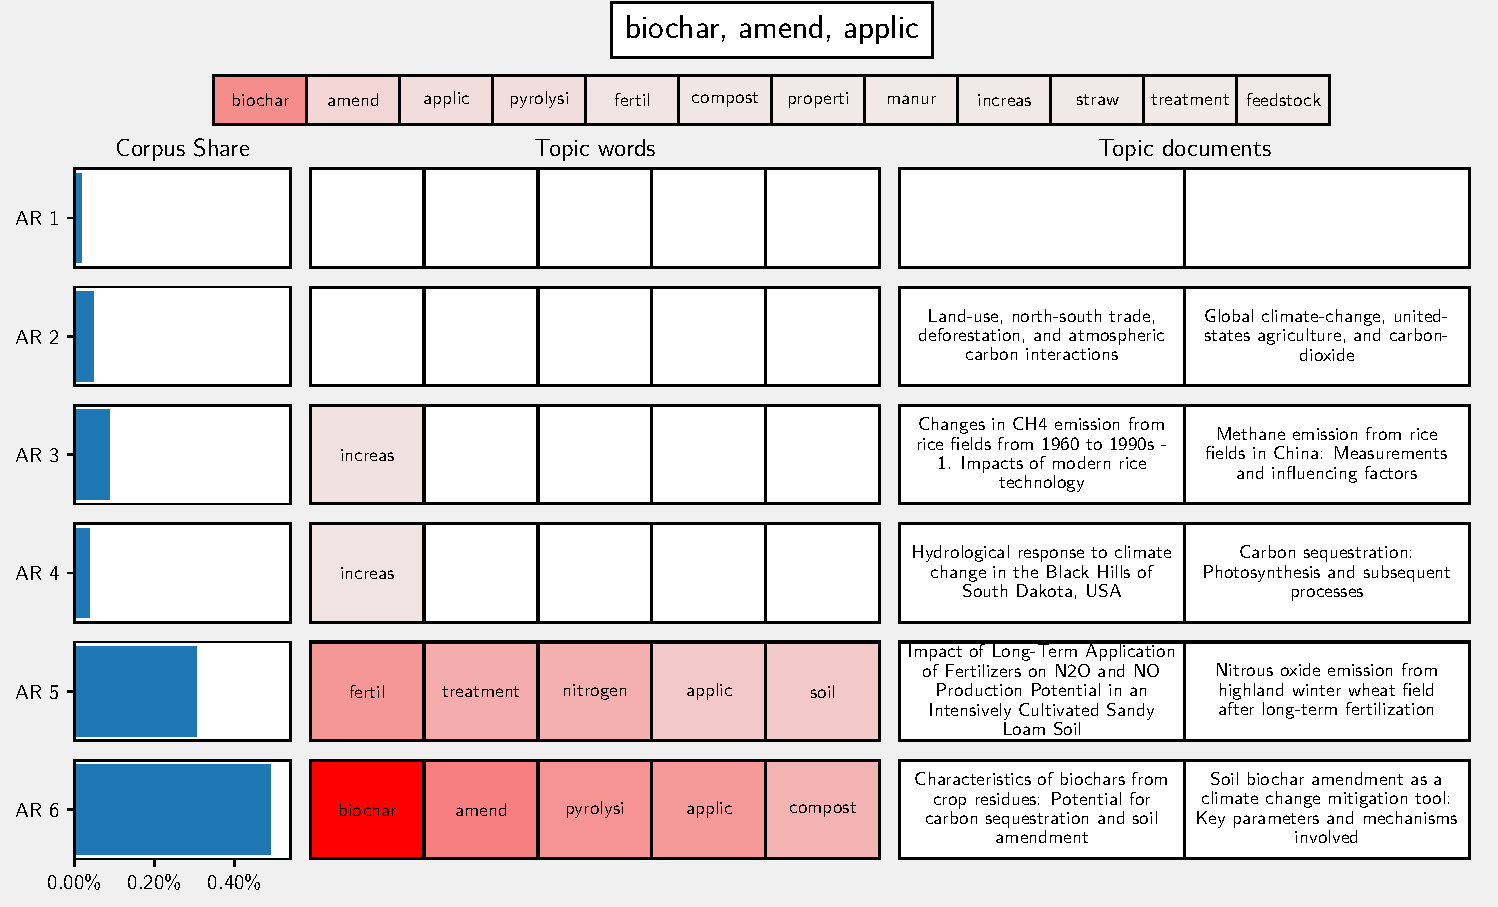
\includegraphics[width=1\linewidth]{plots/single_topic_3_11020.pdf}
		\caption{SI Word and document development of the ``Biochar'' dynamic topic}
		\label{}
	\end{center}
\end{figure}


\begin{figure}
\begin{center}
	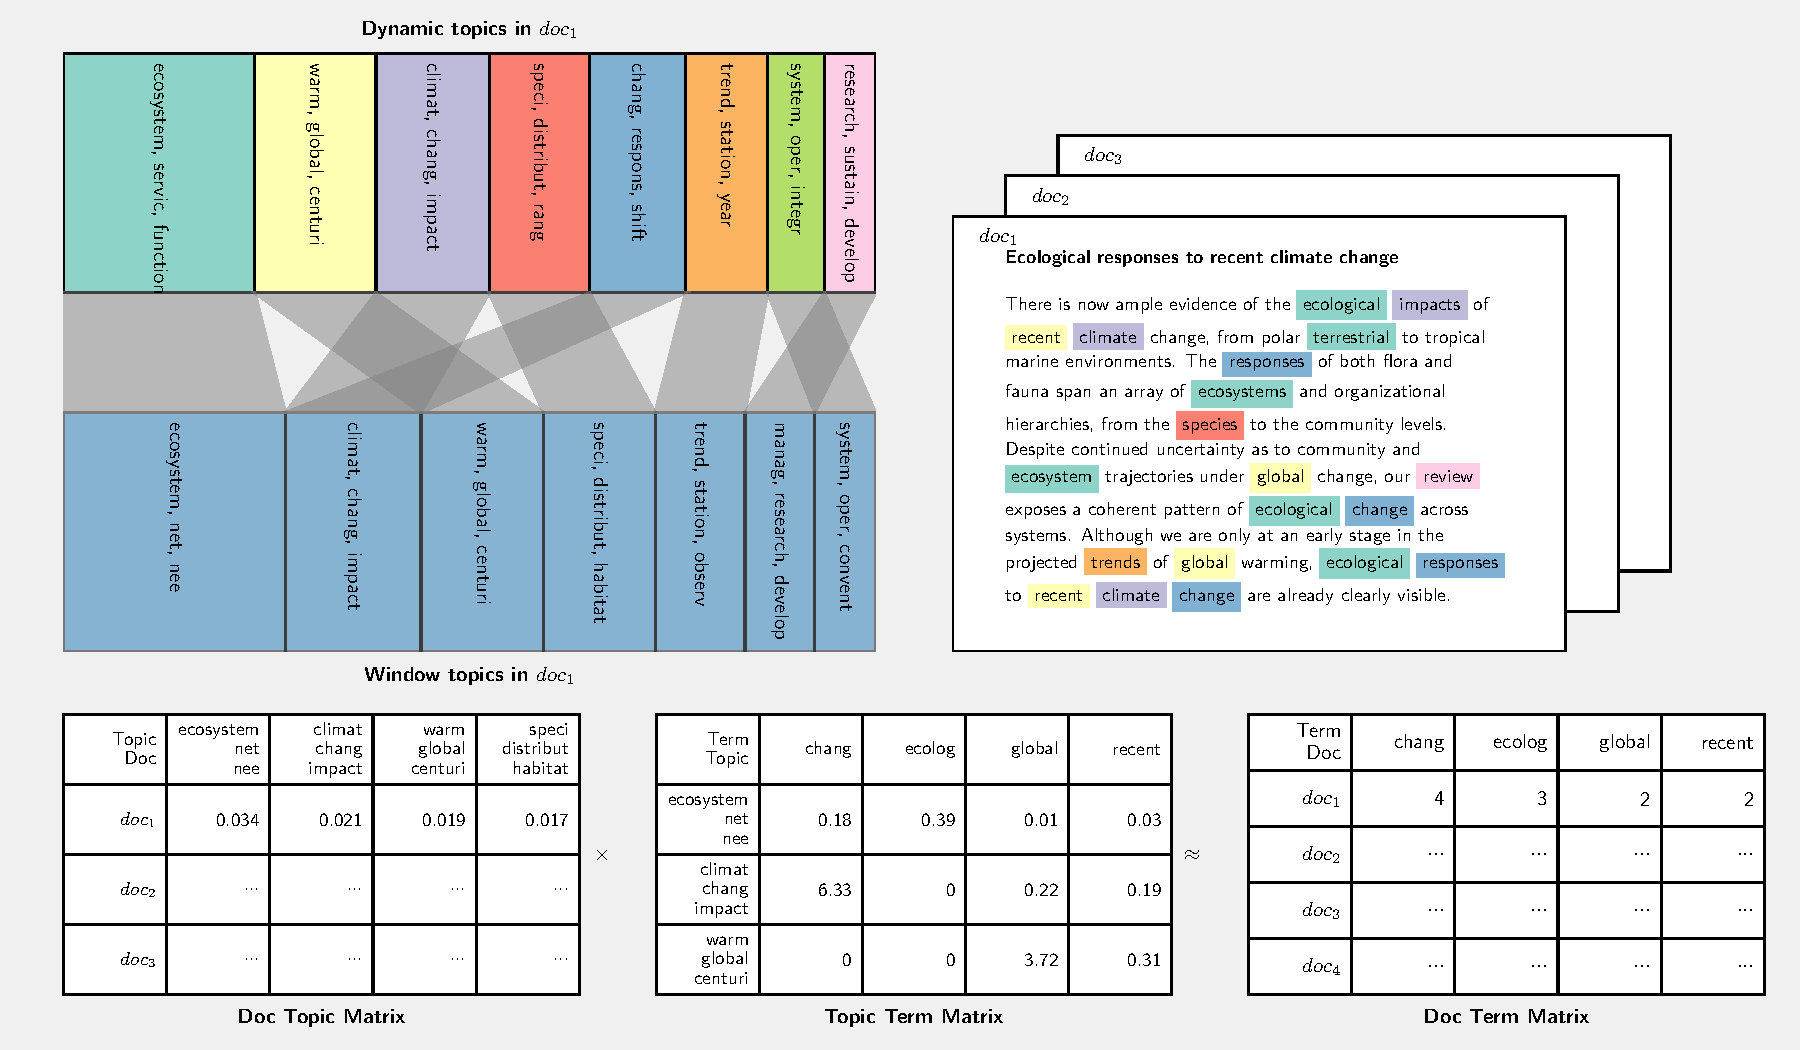
\includegraphics[width=1\linewidth]{plots/single_doc_3_536594.pdf}
    \caption{SI Topic make up of a single document}
    \label{}
    \end{center}
\end{figure}

\bigskip
\noindent\textbf{Physical science topics tend to be the oldest, and the most well represented topics}

\bigskip
\noindent\textbf{Adaptation and impact studies have seen a lot of growth but are well represented in IPCC reports}

\bigskip
\noindent\textbf{New topics around negative emissions and urban form are very recent and not well represented in IPCC reports.}

Negative emissions in special report on 1.5, demand side chapter in AR6



\section*{Discussion}

\bigskip
\noindent\textbf{Solutions, policies and science}

What do policy-makers mean when they ask for more solutions

\bigskip
\noindent\textbf{Perfect representation is not necessarily desirable, but the skewedness should be known}

There may be good reasons for a topic to be less prominent in IPCC discussions than in the wider scientific literature, and these reasons can only be understood and acted upon by humans, not by machine-reading. Nevertheless, it is desirable that assessment makers are aware of the relationship 

%Increase in the frequency of the use of the term ``solutions'' \citep{jabbour2017},

\section*{Methods}
\label{methods}



\subsection*{Data}
%This study reproduces the query developed by \citep{Grieneisen2011}, which is carried out on Web of Science. Though not exhaustive, it gives a good coverage of 

\end{linenumbers}

%\end{multicols}

\listoffigures
\linespread{1}
\bibliography{Mendeley.bib}
\bibliographystyle{unsrt}

\end{document}

